\appendix
\appendixpage
\addappheadtotoc

\section{Naïve Designs} \label{NaiveDesigns}

\subsection{Control a car through gestures} \label{nd1}
\subsubsection*{Naïve Design}

\begin{figure}[h]
\centering
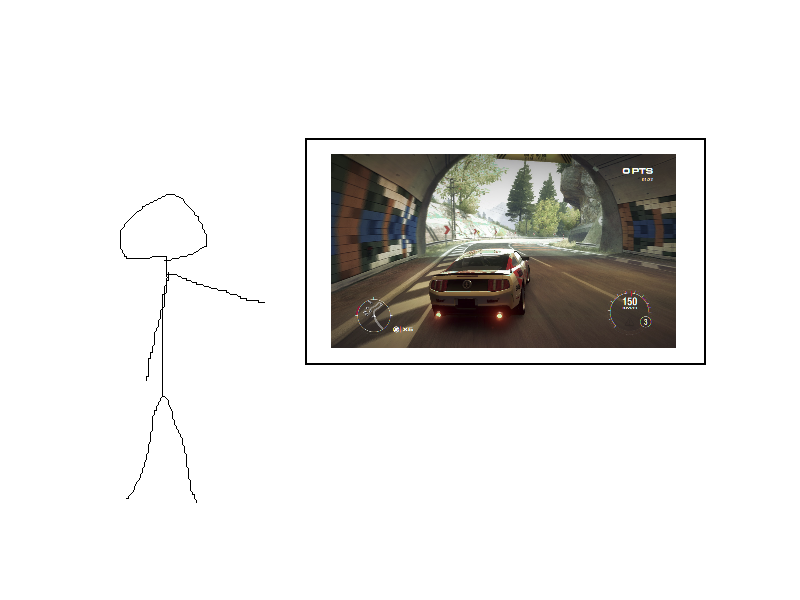
\includegraphics[width=5.5in]{NDesign1}
\caption{}
\label{fig:ndesign1}
\end{figure}

For this design we will use a standard webcam found in most laptops and other types of cameras that can send images to a computer. The idea is to make a vehicle controller, out of a camera, that can react to a user’ hand gestures and translate that into input for a vehicle based application or game. These gestures would translate to tasks commonly used in relation to vehicles, like speed up, slow down, change gears, hand breaking. The system should also be used to control the vehicles directions.


The idea here is to use hardware to get input from the user, however this hardware should not be specialized for gesture recognition, like a Kinect or Eyetoy. The hardware should be common to most computer users. The user should only need to install a piece of software and be ready to use gestures.


To make the camera recognize the different gestures some software will have to be implemented. This software will need to recognize the outline of the user and translate the gestures made by the user into commands for an application. The software should be able to recognize both static and moving gestures, for example, a static, flat hand shown to the camera could translate to a handbrake, or a fast movement of the right arm could translate to a hard turn to the right.

\subsubsection*{Design Analysis}
\noindent\textbf{Motivation} \newline
The motivation behind this concept is to replace the standard ways of using controllers with methods that does not require semi-expensive specialized hardware to operate.

This can be used to control applications like driving games without the need for specialized driving wheels, or analog joysticks, requiring only a basic set of hardware already available to most people who own a laptop. 
\bigskip

\noindent\textbf{Strengths and weaknesses} \newline
Strengths:
\begin{itemize}
\item This can make a driving game more approachable.
\item This can make a driving game controller less costly.
\end{itemize}
Weaknesses:
\begin{itemize}
\item Precision is very important. We do not want to end up in a ditch.
\item Input is not ergonomic.
\item Input lag becomes a much bigger concern.
\item Input methods are not intuitive.
\end{itemize}
\bigskip

\noindent\textbf{Target group} \newline
The primary target group for this concept is people who are confined to using specialized hardware for certain applications, like driving games or equally like-minded applications.
\bigskip

\noindent\textbf{What do you know / need to know} \newline
For this concept a good understanding of image processing is key. The product will be based on image processing to get its readings and translate into input. Precision is key to this product because it will potentially be used for precision operations like navigating a vehicle around a sharp turn.

We need to know how to translate data from a camera into input that the supported applications can understand and use.
\bigskip

\noindent\textbf{What to investigate} \newline
The main focus of the investigations is to figure out how much of this is possible and how much of it is possible using a standard webcam. We need to investigate if it is possible to get accurate readings from a camera that is reliable enough to be usable.
 
Another area of investigation is the industry’ perception of the idea. Is it even a good idea?

We need to know if the ergonomics of this approach is sustainable.
\bigskip

\noindent\textbf{Initial prototype / mock – up.} \newline
An initial prototype could involve using markers on the hands of the user and use one or more cameras to capture data. Software will be needed to translate the input, as well as a demo application involving navigation will be needed. This prototype will be used to answer what is possible with this concept and what needs improving. 

\pagebreak

\subsection{Controller blocks} \label{nd2}
\subsubsection*{Naïve Design}

\begin{figure}[h]
\centering
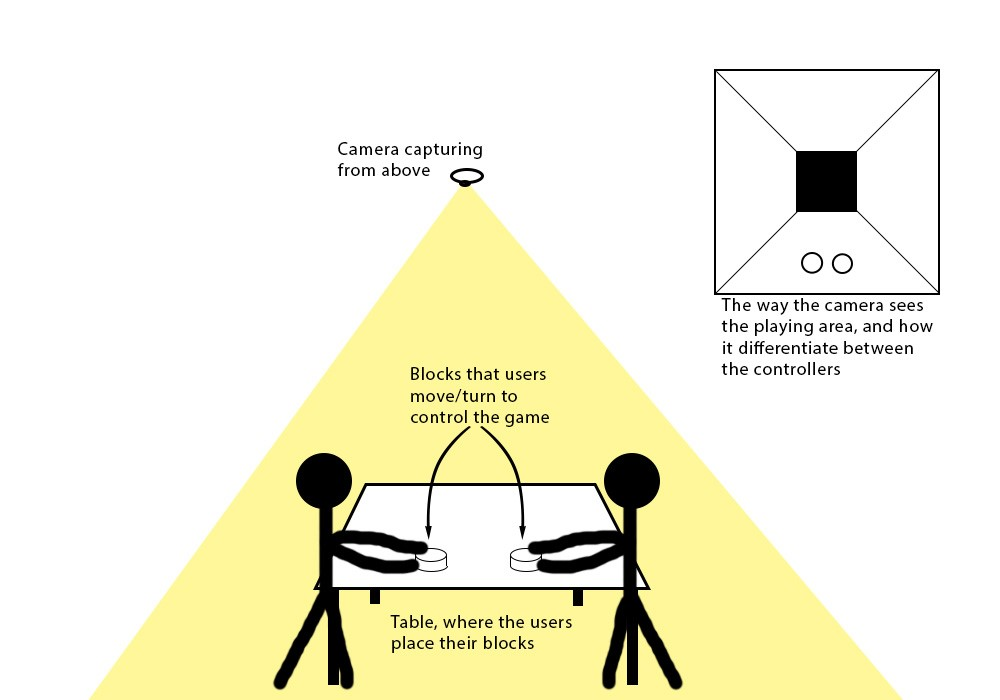
\includegraphics[width=5.5in]{NDesign2}
\caption{Game controller using blocks. By moving and/or rotating the blocks, the user can control the vehicle in the game.}
\label{fig:ndesign2}
\end{figure}
This idea would give the possibilities to both play as a single player and multiplayer (coop and versus). If we say that we are playing a car racing game, then we would use 2 blocks for each car that has to be controlled in the game. This means that one or two players can control each car. By moving the blocks around, the camera can detect their placement and then use this information to control the car in the game. If we have a table we are playing on, the camera would be looking down at the table from above. In the top right of figure \ref{fig:ndesign2} is illustrated how the camera could split up the playing field (where the users are moving the blocks around in) and in this way distinguish between which blocks control what car.

The control blocks would work e.g. as follows:
\begin{itemize}
\item Both blocks forward: the car accelerates
\item Both blocks back: the car brakes
\item Left block forward, right backwards: car turns to the right (and vice versa)
\end{itemize}
For other games that are not car racing, the blocks could be colored. With this addition, you could also rotate the blocks, which the camera could register by the colors on the blocks.

\subsubsection*{Design Analysis}
\noindent\textbf{Motivation} \newline
\noindent\textbf{problem} - This idea is based on a way to make a gaming platform, if you will, cheap, compared to other professional and popular platforms such as the Nintendo Wii, and Xbox Kinect, which both tracks movement performed by a user.
\bigskip

\noindent\textbf{Opportunities} - The idea here would give the possibility to play together (or against) your friends, as you can play multiple players at the same time. You can cooperate as two (or maybe even more) players in controlling one vehicle in the game, if you would like. This possibility is obtained by using two or more blocks on the board to control each vehicle.
\bigskip

\noindent\textbf{Inspiration} - The source of inspiration came partly from the previous idea (Race-making Game) where you are using blocks or something alike, to tell e.g. the car when to turn. An additional source of inspiration was the “music board” where you are using different kinds of blocks, and by placing them on a surface, you create different kinds of sounds. 
\bigskip

\noindent\textbf{Strengths and weaknesses} \newline
Strengths:
\begin{itemize}
\item Options for multiplayer gaming as well as single player
\item Cheap: only a webcam is needed, the blocks can be homemade
\item The blocks can both be moved around and rotated, giving several ways of controlling the vehicle
\item Social gathering, as the idea is to gather more people around the table and play together in the same room.
\end{itemize}
Weaknesses:
\begin{itemize}
\item Camera placement can be a bit problematic: camera has to see the blocks from above
\end{itemize}
\bigskip

\noindent\textbf{Target groups} \newline
As the main problem is focused on making a gaming controller of some kind, so target group will primarily be people already playing video games. This does not necessarily mean hard-core gamers. In fact, non-hard-core gamers would be of preference. Initially this idea might seem more appealing to the same kind of people that uses Nintendo Wii, Xbox Kinect or alike, as this idea involves having people in the same room when playing. Those kind of people might be families playing together once in a while, or friends gathering to play together in another way than LAN parties.
\bigskip

\noindent\textbf{What do you know / need to know more about?} \newline
\noindent\textbf{Visual computing} - Some knowledge needed to make this idea come true would be how visual computing actually works. The camera in this idea would need to recognize the blocks on the table and read how they are being manipulated to perform an action in the game. 
\bigskip

\noindent\textbf{Users} - The product of this idea especially has to be appealing to the target group in order to give them the satisfaction they would have gotten from using a popular gaming platform. This means that the controls have to be easily understandable and manageable as well as many other things, which would need research.
\bigskip

\noindent\textbf{SOTA} - At the moment it is unknown if there are ideas like this already developed. So far it is known that there is a device that utilizes something like this idea, but instead of controlling a vehicle in a game, the device provides sound and music according to what kind of block you place on a surface that reads the blocks.
\bigskip

\noindent\textbf{What would you be investigating?} \newline
\noindent\textbf{Image analysis and processing} - 
Using a webcam will provide a flow of images of the area in which the users will be controlling their blocks. These images need to be analyzed and processed in order for the software, that will be developed, to understand what the user wants the program to do. To be able to use the images like this research has to be done in the area of image analysis and processing.
\bigskip

\noindent\textbf{Initial prototype} \newline
For an initial prototype, it would be useful to focus on using one specific video game. Say we take a car racing game; the prototype would only have to focus on how to control a car in order to see if it is even possible to get near a product where the user would be able to control all kinds of vehicles.

\pagebreak

\subsection{Immersive Racing Game Experience} \label{nd3}
\subsubsection*{Naïve Design}
\begin{figure}[h]
\centering
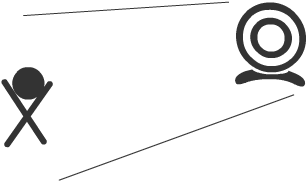
\includegraphics[width=5.5in]{NDesign3}
\caption{}
\label{fig:ndesign3}
\end{figure}
The theory behind (IRGE) is to use a static webcam to track your movement/face by recognition and thereby allowing enhanced immersive gameplay by the use of real like movement as required in the specific computer game.


By tracking the whole body you are able to navigate in the game, since we are going to make a vehicle controller based on the user we got many possibilities. We might focus on car games it would be obvious make the webcam track our movements like we were driving a real car. If time is on our side we might also make a controller for other kind of vehicles. 


This use of webcam movement tracking can generally be used in games that requires varied movement such as Racing games, First person shooters, puzzle games(Portal) and others, where the player act as a person with movement functionalities within the game itself.

\subsubsection*{Design Analysis}
\subsubsection*{Motivation}
Also as several of the other ideas the motivation for this one is not based on a particular problem that can be solved. Hence it is an idea that is specifically targeted for entertaining purposes only.


The theory is to enhance immersive gameplay by the use of real life movements in the specific computer game, where it is required.


The opportunity with this idea is to enhance the experience by being the subject which is used to control the in-game player in terms of movement.


\subsubsection*{Strengths and weaknesses}
Strengths:
\begin{itemize}
\item Could contribute to the already evolving technology of virtual reality.
\item Would be a cheaper alternative to more complicated ways of immersion, such as the Wii, provided that the user has enough space.
\item Healthiness. The user is able to get some sort of exercise while playing a game.
\item Could be a multiplayer experience.
\item Has the potential to be fun to make.
\item Has the potential to be fun for the users, although that would be subjective.
\end{itemize}
Weaknesses:
\begin{itemize}
\item Requires a large amount of space to interact in.
\item Could limit social aspect of games.
\item Most people do not have the required equipment and space to make this game fully functional.
\end{itemize}


\subsubsection*{Prototype - Mock-up}
An early prototype for this concept could be a hallway with a screen and a webcam at the end. In the hallway could be obstacles that the user can hide behind as part of a game. Software will have to make to be made to translate the data from the camera into input to a demo game that we will borrow for the testing.
\bigskip

A prototype would clarify if users would like the idea of a racing game controlled by movements. A prototype could help show the technical limitations of this concept.


\subsubsection*{Target Groups}
The ideal target group for this solution is people who like to play games, but feel that the control options available are insufficient / uninspiring, and would like the games to be more immersive.


\subsubsection*{What do we know / what do we need to know more about}
We know that the concept is somewhat similar to that of the Kinect as far as movement goes. The innovative part of the concept is that the player will be able to see himself on the monitor, and will be able to drive the car around by using steering wheel movements, speed up and down movements and other kind of movements that are needed to control the car or options in the game.
\bigskip

The Kinect is a state of the Art product in this line of gaming, so it will, for obvious reasons, is natural to investigate how it works.


\subsubsection*{How much research has to be done in this area (from 1-5, where 5 is most)?}
\begin{itemize}
\item State of the Art: 4
\item Full body motion capture: 5
\item Perception: 2
\item Player motivation: 5
\end{itemize}


\subsubsection*{Investigations}
For the user to be able to control the game via the webcam, a study upon how you analyze and process an image input from the camera has to be done. The focus here will be how to find and analyze an object/person in the picture and use the person’s movements and gestures to apply some action in the game.

\pagebreak

\subsection{Pointing controller} \label{nd4}
\subsubsection*{Naïve Design}
\begin{figure}[h]
\centering
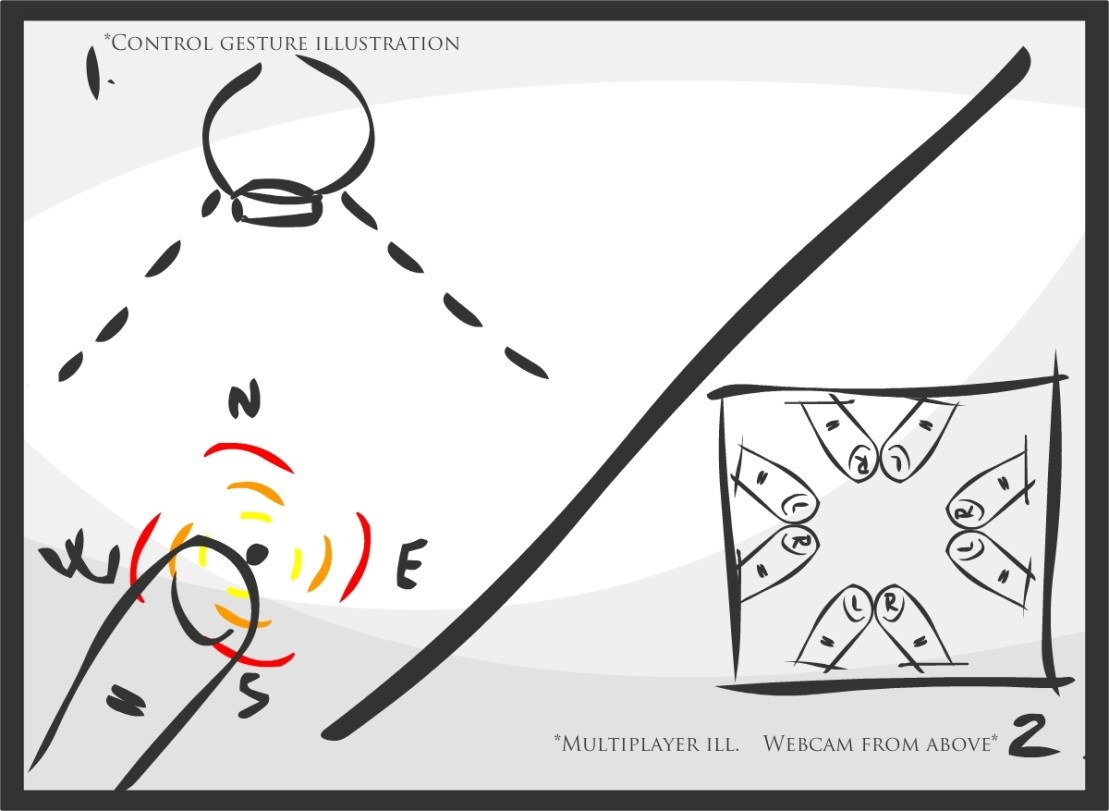
\includegraphics[width=5.5in]{NDesign4}
\caption{}
\label{fig:ndesign4}
\end{figure}

The idea behind this concept is to use a webcam to track finger(s) on a plain surface to register movement and functionalities of the designated game. By relocating the finger(s), depending on the game, the input will act accordingly to the specific game/functionality.
\bigskip

Also, to incorporate multiplayer functionality, several players can be recognised and because of limited movement to control the specific game, a single webcam would be adequate to keep track of (x) players.
\bigskip

Illustrates the finger movement, and predetermined possible movement/control functionalities of the setup. (Illustration \ref{fig:ndesign4}: Example 1)
\bigskip

The rotation of the players, can be adjusted down to the individual to address the angle of the screen and the angle of control that the specific player so desires. (Illustration \ref{fig:ndesign4}: Example 2)


\subsubsection*{Naïve Design}
\subsubsection*{Opportunities}
The idea is based on visual computing where there is no need for controllers. A simple webcam and a plain surface will suffice to create the specified game experience where you control the functionalities with the tip of your finger(s). This method of controlling the vehicle can be modified to combine alternative methods of controlling the game, but also customization of alternative controlling methods possible since there are buttons to limit the possibilities.

\subsubsection*{Strength/Weakness}
The \textbf{strength} of the design is first of all the simple hardware requirements which is easy accessible and plausibly with a very simple setup. 
\bigskip

Also, by not limiting ourselves to a controller which is already developed with a limited amount of functionalities, we are able to imitate all of the preexisting functionalities and exceed those, since there are no button limits, but rather space limit depending on the single player/multiplayer experience.
\bigskip

The \textbf{Weakness} of the design is that by utilizing a camera for tracking movements, you do not get any sort of haptic feedback under any circumstances during the experience.
\bigskip

Also, it is possible that the amount of functionalities that must be present in order to be comparable in terms of functionalities with other game platforms, is too much to cope with, since there are no visual interface lying on the surface while you are playing. Only a visual interpretation of the game mechanics that might appear on the screen.

\subsubsection*{Target groups}
The target group is people whom are interested in playing vehicle games on consoles and plausibly already do so. Preferably we are able to aim at people who are actually playing/performing vehicle gaming on a higher level, in order to research whether or not our take on a plausible alternative to preexisting methods is even a possible solution.

\subsubsection*{What to know}
\noindent\textbf{Theory/Research} - First of all we need to figure out what makes a vehicle game the preferred experience with the different controllers in order for us to establish requirements towards, what our product should be able to do and contain.
\bigskip

Furthermore, we need to establish a base of knowledge of the vehicle games in order to figure out which functionalities our product should have. Lastly, we must of course research on how to create such controller for it to be able to function to a plausible large number of games, where the controller would be equally efficient as the preexisting. 
\bigskip

\noindent\textbf{Theory/Research}\newline
\noindent\textbf{Users} - First of all we must establish criteria towards what the users think that the product would need in terms of design and functionality. Also, it would be plausible that the users are so used to “regular” controllers when playing vehicle games, so perhaps, also try a separate target group of people who do have non to little experience with vehicle games to establish a measurable amount of data of the user experience within both groups.
\bigskip

\noindent\textbf{SOTA} - The state of the Art within this matter is the pre-existing controllers on the market. The Kinect controller, the PS controller, Wii and the special developed wheels to emulate the driver experience.

\subsubsection*{What to investigate}
First of all we must investigate the image processing technology behind the idea. What we are able to do and how we can utilize that specific technology.
\bigskip

Next we must investigate the preexisting controllers to delimit ourselves to how we can make the product “comparable with other gaming platforms”. What should our product we able to do, can it be implemented, and how can we improve on the matter?

\subsubsection*{Prototype}
The prototype would most likely be an alternative to the pre-existing controllers in terms of key-functionality. We could possibly argue that we have created an alternative method of controlling vehicle games, but since it’s a different approach – there would be both advantages and disadvantages which would probably be evaluated individually by the test subjects of the evaluation.
\bigskip

The success criteria would be if the product would suffice when comparing the established requirements and still be functional to a satisfaction of the users, but that cannot be speculated upon before the specific requirements for the success criteria is established.

\pagebreak

\subsection{Object-controlled Visual Processing} \label{nd5}
\subsubsection*{Naïve Design}
\begin{figure}[h]
\centering
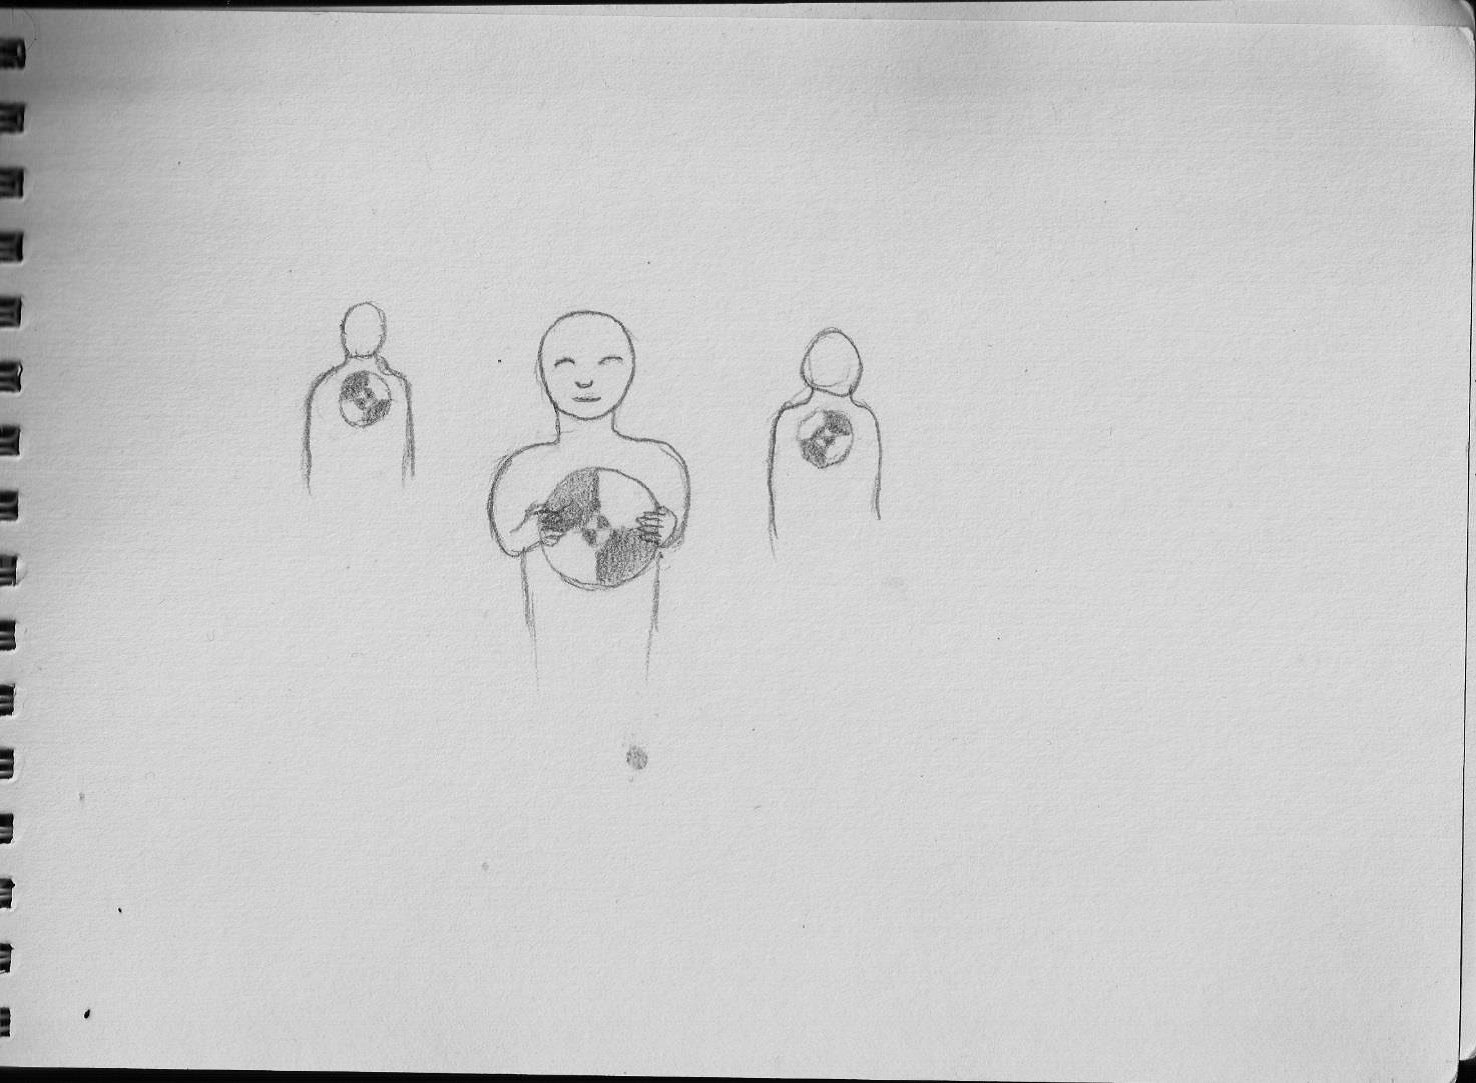
\includegraphics[width=5.5in]{NDesign5}
\caption{}
\label{fig:ndesign5}
\end{figure}

The idea revolves around a multicolored - or shape-recognizable object that can be moved around in front of the webcam to create a motion capture-device that can be used as a logical vehicle controller e.g. a plate as seen in the image for controlling a car or boat etc.
\bigskip

The objects are going to have some sort of pattern on them to make them easier recognizable for the camera. Due to this pattern, it should be easy for the camera to pick up side-to-side as well as up-down movement, rotation, and forwards and backwards movement. It also makes it easy for several people to use the device at the same time, allowing for potential multiplayer games, or collaborative work.
\bigskip
 
The currently State-of-the-art products out there such as Kinect, PlayStation Move or Wii only allows for 2-3 players simultaneously. So maybe we will be able to create a cheap alternative to those optional products that are furthermore able to sustain more players. Maybe we could also enable multiplayer online, so people might be able to pick up their plate and join the game with an avatar that reacts to the object’s movement.
\bigskip
	
In order to make this, knowledge about image processing needs to be known. However because the pattern the camera should recognize is a pre-defined static object, it should prove less of a challenge than with a varying object such as a human hand.

\subsubsection*{Design Analysis}
\subsubsection*{Motivation}
The concept behind this idea, is replacing the traditional mouse, with a wireless (and powerless) solution to be able to play vehicle games in an interactive, logical and intuitive fashion. 

We are motivated by the fact that products such as the Wii or Kinect seldom can sustain more that 2-3 players, and usually only come with 2 controllers, extra controllers can be purchased, but they usually cost a lot.

\subsubsection*{Strengths / weaknesses}
Strengths:
\begin{itemize}
\item Conceptually, the user would be able to use this 'mouse' from a rather great distance (though with diminished accuracy, as a side effect).
\item The physical aspect of the mouse could simply be a sticker, or something similar carrying a 	specific pattern, thus removing the need for a power source.
\item The number of players could be limited only by the restrictions of the game.
\end{itemize}
Weaknesses:
\begin{itemize}
\item The accuracy of the device is highly dependent on the skills of the user
\item Depending on the quality of the webcam, distance could very quickly become an issue for 	accuracy, as coding can only do so much.
\end{itemize}

\subsubsection*{Target groups}
The target group could be anyone who are interested in playing interactive games. 

\subsubsection*{What do you know / what do you need to know?}
For this product, a strong knowledge of image processing is key:
\bigskip

A) Knowledge of how to capture, record and convert a specific pattern (like the ones in the illustration) is required, in order for the program to reliably record the movement of that specific object, and not random background objects.
\bigskip

B) Knowledge of converting the data from A) into movement on the computer screen is needed - This could further be expanded upon, to allow for different settings (for different programs).

\subsubsection*{What would you be investigating?}
The main focus would be investigation regarding image capturing and processing.
\bigskip

Additionally we would need to gather some information regarding how web cams work, how the different types differ from one-another, and how this will affect the program - And how (if possible) to counteract this.
\bigskip

Networking would also be required to investigate if we were to implement an online solution. 

\subsubsection*{What could be an initial prototype / mock-up?}
An initial prototype / mock-up are not easy to make, as the solution is rather simple. One solution, however, could be to create a functional program, with only limited actions available (such as simply moving the mouse around, using image capturing.

\pagebreak

\subsection{Race-making game} \label{nd6}
\subsubsection*{Naïve Design}
\begin{figure}[h]
\centering
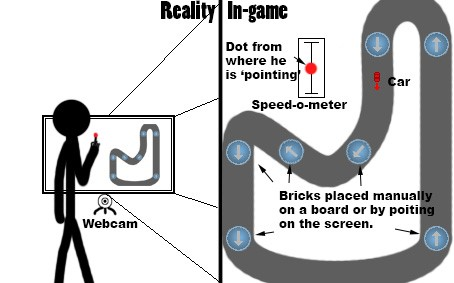
\includegraphics[width=5.5in]{NDesign6}
\caption{}
\label{fig:ndesign6}
\end{figure}

This idea is inspired by some of the racing tracks made for kids to build. You put the track together, and then you had a controller that could only control the speed of your car and nothing else. The goal was then to try and keep your car on the track, while still going at a maximum speed.
\bigskip

Of course what we should be explaining here is the controller, not the game itself. The controller has a board (not in the above picture), where you place down the bricks as “points” where you would like the track to go. The game then connects these points with lines, and there you have the track! This would use image processing to figure out where the bricks were placed.
\bigskip

You then use your finger to control the speed of the car, trying to make it go fast, but not too fast. You need to put a colored thing on your finger so the camera can see where it is placed.
\bigskip 

Note that this idea could be combines with some of the next ideas explained, and the control schemes could be altered to give you more control of the car.

\subsubsection*{Design Analysis}
\subsubsection*{Motivation}
This idea has roots in our childhood, and because of that it is something that we can relate to.
\bigskip

The game itself isn’t too complicated, with the hardest part probably being how to connect the dots to form a track, and making the car controls feel nice. The image processing part of it should be fairly simple.
\bigskip

This idea could also potentially require us to build a table of some sort for the bricks to be placed on. This means that there will also be some work in creating something physical, which some group members might like.

\subsubsection*{Strengths/weaknesses}
Strengths:
\begin{itemize}
\item The idea is something we can relate to.
\item Could be cheaper than buying an actual racing track.
\item Allows users to be creative by being able to create their own things with the provided material.
\item The idea itself is fairly simple.
\item Allows for social interaction.
\end{itemize}
Weaknesses:
\begin{itemize}
\item Could potentially require 2 cameras, however this can be fixed by using the board where you place the bricks as the “control-space” as well.
\item We’re not sure yet exactly how we can give the user the ability to create the track themselves yet.
\item Requires quite a bit of programming, might not be fun for all members.
\end{itemize}

\subsubsection*{Target group}
The target group would be anyone who plays games. Younger people might be a greater target group however, since they might’ve played the physical version of the game, and has some nostalgia when it comes to the game.
\bigskip

The game should be really simple and intuitive to use, so you don’t need a lot of technological expertise to use the product.

\subsubsection*{Knowledge}
We know for a fact that some students have made tables that are able to detect objects on top of it before, so some research has already been done in this area, and we’ll have some other products to compare ours to. The same has been done with color recognition.
\bigskip

In order to create this idea, we would need knowledge about image processing to create the controlling features. We would also need knowledge about how to create the actual game. This could be done in a lot of programs such as Unity, Flash, Processing and more. We could potentially also create it from scratch using c++, however this would most likely not be preferred.
\bigskip

We also need knowledge about vectors and vector calculation in order to create the track, and some knowledge about 2d physics, to make the car act in a way we want. However a program such as Unity already has a physics engine, potentially saving us time.
\bigskip

We can make loads of prototypes of this idea, and it has a lot of “steps” on which we can test the game. We can test the initial color recognition without the need of anything else, we can test the creation of the track without the need of anything else, and we can test the car ‘mechanics’ in a way without the need of much, except a track to follow.

\pagebreak

\subsection{Tabletize your computer!} \label{nd7}
\subsubsection*{Naïve Design}
The idea for this design is, using a standard webcam, simulating the rotation measuring devices of modern tablets and smart phones, allowing computer users the same intuitive means of controlling games.
\bigskip

As the webcam is recording, edges will be recognized (using image processing), and the movement of said edges will be converted into movement on the computer - In other words, movement within the captured pictures will be replacing the tilting sensors of the tablets and smart phones.

\subsubsection*{Design Analysis}
\subsubsection*{Motivation}
The motivation behind this concept, is to create software, that will allow a webcam to replicate the tilting and rotation sensors ordinarily found in e.g. tablets and smartphones. This would allow desktop and laptop computer users to immerse them selves in similar games - ie. games where the controls are more intuitive than simply using the WASD movement keys, for example.

\subsubsection*{Strengths and weaknesses}
Strengths:
\begin{itemize}
\item Allows for a more immersive experience
\item Expands the range of games available to computer users even further.
\item Could possibly be utilized for other purposes, where a tilt sensor could be useful.
\end{itemize}
Weaknesses:
\begin{itemize}
\item Hardware not built for this kind of action, unless using an external webcam.
\item Potentially hard / impossible to do general calibration, causing the device to needing 	recalibration after either every  game session or after every time it is moved from location to 	location.
\item Unless using external webcam, the setup can be both heavy and cumbersome, making the 	device less intuitive than the alternative, thus defeating the point.
\end{itemize}

\subsubsection*{Target group}
What do we know / what do we need to know more about:

We will most likely be using openFrameworks (C++ coding) to process the images into movement data. What we need to know is, how to convert the stream of images from the webcam into usable movement data ( ie. how to detect the movement in the images reliably). Furthermore we need to convert this data into actual movement in a game.

\subsubsection*{Investigation}
We will need to investigate similar, professional, solutions - sort of like the tablets and smartphones, but we should try to see if we can find someone who have done the same - without the use of tilt-sensors.
\bigskip

We will need to research a lot of image processing, and figure out how we're going to approach the movement - record - movement process (ie. recorded movement -> data -> output movement), and how much movement should account for how much movement on screen. 

\subsubsection*{Initial prototype}
An initial prototype is not easy to do, as it is highly software based, and thus will more or less be finished, once an initial prototype is ready for testing. "Simulations" (or Wizard of Oz-experimentations) could be used, however, as this would give us some idea of how the program will work and feel for the users, while being very time efficient.
